
%----------------------------------------------------------------------------------------
%	PACKAGES AND OTHER DOCUMENT CONFIGURATIONS
%----------------------------------------------------------------------------------------

\documentclass[paper=a4, fontsize=12pt]{scrartcl} % A4 paper and 11pt font size
\usepackage{graphicx}
\usepackage{wrapfig}
 \usepackage{float}
\usepackage[T1]{fontenc} % Use 8-bit encoding that has 256 glyphs
\usepackage{fourier} % Use the Adobe Utopia font for the document - comment this line to return to the LaTeX default
\usepackage[english]{babel} % English language/hyphenation
\usepackage{amsmath,amsfonts,amsthm} % Math packages
\usepackage{sectsty} % Allows customizing section commands
\allsectionsfont{\centering \normalfont\scshape} % Make all sections centered, the default font and small caps
\usepackage{color}
\usepackage{fancyhdr} % Custom headers and footers
\pagestyle{fancyplain} % Makes all pages in the document conform to the custom headers and footers
\fancyhead{} % No page header - if you want one, create it in the same way as the footers below
\fancyfoot[L]{} % Empty left footer
\fancyfoot[C]{} % Empty center footer
\renewcommand{\headrulewidth}{0pt} % Remove header underlines
\renewcommand{\footrulewidth}{0pt} % Remove footer underlines
\setlength{\headheight}{13.6pt} % Customize the height of the header

\numberwithin{equation}{section} % Number equations within sections (i.e. 1.1, 1.2, 2.1, 2.2 instead of 1, 2, 3, 4)
\numberwithin{figure}{section} % Number figures within sections (i.e. 1.1, 1.2, 2.1, 2.2 instead of 1, 2, 3, 4)
\numberwithin{table}{section} % Number tables within sections (i.e. 1.1, 1.2, 2.1, 2.2 instead of 1, 2, 3, 4)
\usepackage{color}
\definecolor{dkgreen}{rgb}{0,0.6,0}
\definecolor{gray}{rgb}{0.5,0.5,0.5}
\definecolor{mauve}{rgb}{0.58,0,0.82}
\setlength\parindent{0pt} % Removes all indentation from paragraphs - comment this line for an assignment with lots of text
\usepackage{listings}
\lstset{ %
  language=Matlab,                  % the language of the code
  basicstyle=\footnotesize,       % the size of the fonts that are used for the code
  numbers=left,                   % where to put the line-numbers
  stepnumber=1,                   % the step between two line-numbers. If it's 1, each line 
                                  % will be numbered
  numbersep=5pt,                  % how far the line-numbers are from the code
  backgroundcolor=\color{white},  % choose the background color. You must add \usepackage{color}
  showspaces=false,               % show spaces adding particular underscores
  showstringspaces=false,         % underline spaces within strings
  showtabs=false,                 % show tabs within strings adding particular underscores
  frame=single,                   % adds a frame around the code
  rulecolor=\color{black},        % if not set, the frame-color may be changed on line-breaks within not-black text (e.g. commens (green here))
  tabsize=4,                      % sets default tabsize to 2 spaces
  captionpos=b,                   % sets the caption-position to bottom
  breaklines=true,                % sets automatic line breaking
  breakatwhitespace=false,        % sets if automatic breaks should only happen at whitespace
  title=\lstname,                 % show the filename of files included with \lstinputlisting;
                                  % also try caption instead of title
  keywordstyle=\color{blue},          % keyword style
  commentstyle=\color{dkgreen},       % comment style
  stringstyle=\color{mauve},         % string literal style
  escapeinside={\%*}{*)},            % if you want to add a comment within your code
  morekeywords={*,...}               % if you want to add more keywords to the set
}

% this is needed for forms and links within the text
\usepackage{hyperref}
%----------------------------------------------------------------------------------------
%	TITLE SECTION
%----------------------------------------------------------------------------------------

\newcommand{\horrule}[1]{\rule{\linewidth}{#1}} % Create horizontal rule command with 1 argument of height

\title{	
\normalfont \normalsize 
\huge MechE 416 HW 1 \\ % The assignment title
\horrule{2pt} \\[0.5cm] % Thick bottom horizontal rule
}

\author{Christopher Sims} % Your name

\date{\normalsize\today} % Today's date or a custom date

\begin{document}

\maketitle % Print the title


%----------------------------------------------------------------------------------------
%	PROBLEM 1
%----------------------------------------------------------------------------------------
\section{\small{Data analysis and property calculation}}
\begin{figure}[H]
  \centering
      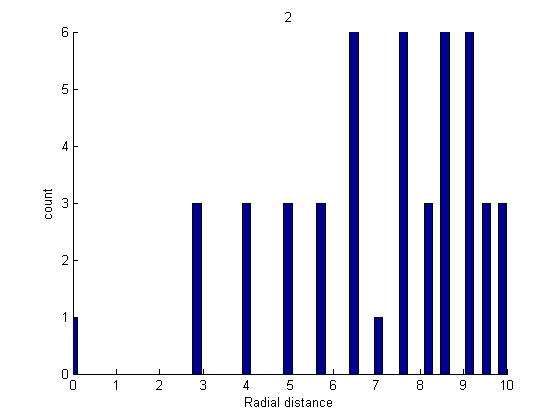
\includegraphics[width=0.8\textwidth]{1.png}
  \caption{a) Solid b) FCC c) Gold }
\end{figure}
R = [1,1.4,1.73]
N = [3,3,3]
\begin{figure}[H]
  \centering
      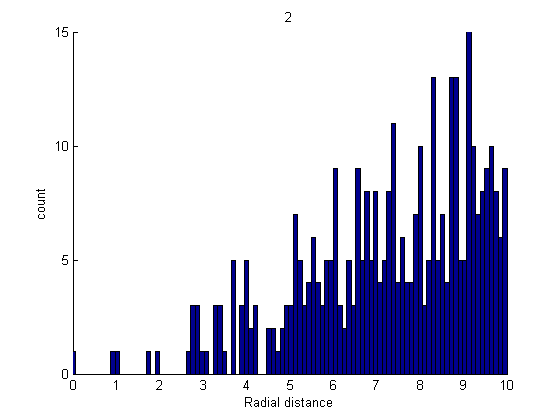
\includegraphics[width=0.8\textwidth]{2.png}
  \caption{a) liquid b) none c) water}
\end{figure}
R = [1,1.11,1.88]
N = [1,1,1]
\begin{figure}[H]
  \centering
      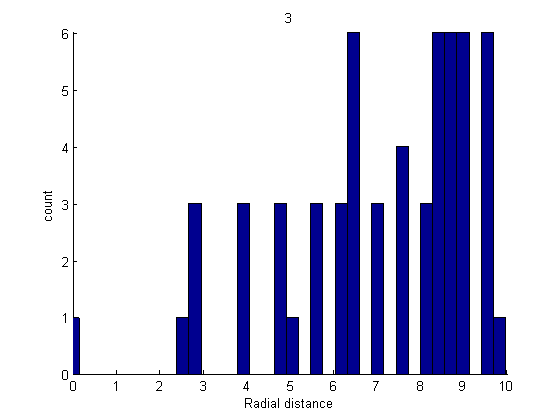
\includegraphics[width=0.8\textwidth]{3.png}
  \caption{a) Solid b) BCC c) Fe}
\end{figure}
R = [1,1.25,1.75]
N = [1,3,3]
\begin{figure}[H]
  \centering
      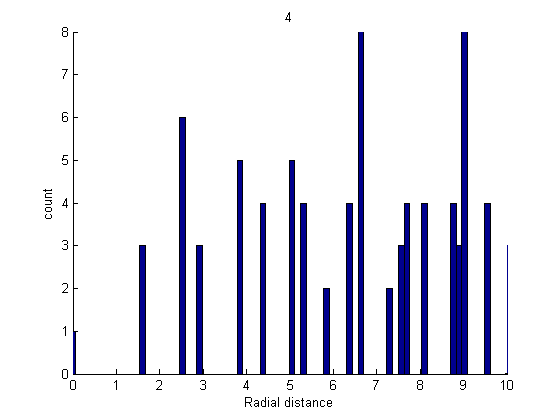
\includegraphics[width=0.8\textwidth]{4.png}
  \caption{a) Solid b) Hexagonal c) Graphene}
\end{figure}
R = [1,1.63,2]
N = [3,6,3]
\begin{figure}[H]
  \centering
      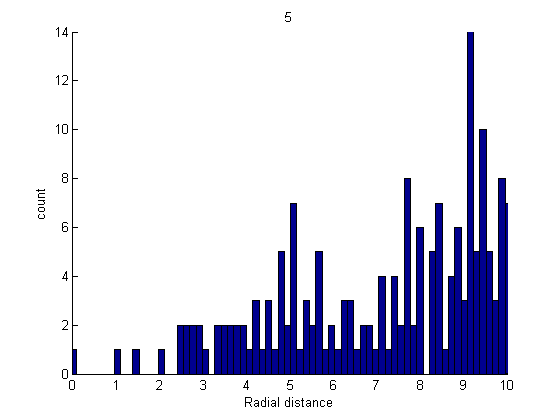
\includegraphics[width=0.8\textwidth]{5.png}
  \caption{a) Solid/liquid? b) none c) Protein}
\end{figure}
R = [1,1.5,2.33]
N = [1,1,1]
I calculated the Ratios for the different crystal systems. To get a vector of values I use histc(). This gives me a vector of values. By using a bin width algorithm I can calculate the crystal distances. I then run an algorithm to calculate the number and location of the atoms. after this I divide the ratios R by my calculated values and where there is a small deviation the the resulting vector i determine that to be the crystal system I am looking for. 

%----------------------------------------------------------------------------------------
%	PROBLEM 2
%----------------------------------------------------------------------------------------

\section{\small{ Elastic properties of crystals modeled using a LJ pair potential}}
%------------------------------------------------
\subsection*{\small{a) Assuming a 12:6 Lennard-Jones potential in an FCC lattice 
write out the expression for the equilibrium position between pairs of atoms.
Using the unit lattice properties of copper, express the LJ length parameter \(\sigma\) as a
function of the lattice parameter \(a0\)}}
\[U(R) = 4\epsilon \Big[\frac{\sigma^{12}}{r^{12}}+ \frac{\sigma^{6}}{r^{6}} \Big]\]
\[\Sigma \frac{1}{r^6} = \frac{14.45}{R^6}\]
\[\Sigma \frac{1}{r^{12}} = \frac{12.23}{R^{12}}\]
\[U(R) = 4\epsilon \Big[\frac{\sigma^{12}}{R^{12}}+ \frac{\sigma^{6}}{R^{6}} \Big]\]
\[\frac{d U(R)}{dR} = 4\epsilon \Big[\frac{12(12.13)\sigma^{12}}{R^{13}} - \frac{6(14.45)\sigma^6}{R^7} \Big]  \] 
\[\frac{d U(R)}{dR} = 0; 4\epsilon \frac{12(12.13)\sigma^{12}}{R^{13}} = 4\epsilon \frac{6(14.45)\sigma^6}{R^7}\]
\[\frac{12(12.13)\sigma^{12}}{6(14.45)\sigma^6} = \frac{R^{13}}{R^7}\]
\[\frac{6(12.13)\sigma^6}{14.45} = R^6\]
\[6(0.839)\sigma^6 = R^6\]
\[\sqrt[6]{6(0.839)\sigma^6} = \sqrt[6]{R^6}\]
\[R = \frac{a_0}{\sqrt{2}}\]
\[1.3\sqrt{2}\sigma = a_0\]

\begin{center}
\boxed{\sigma = \frac{a_0}{1.3\sqrt{2}}}
\boxed{a_0 = 3.97 \dot A }
\boxed{a_0 = 1.83\sigma}
\end{center} 
%%%%%%%%%%%%%%%%%%%%%%%%%%
\subsection*{\small{B) Determine an expression for the minimum potential well of the LJ potential,corresponding to the maximum energy stored in each bond using the expression
for bulk modulus and experimental values for the obtained bulk modulus.}}
\[K = -V\frac{\partial p}{\partial U}\]
\[p = -\frac{\partial U}{\partial V}\] 
\( \mu = \frac{U}{N} ; V_c = \frac{V}{N}\)
\[K = V_C\frac{\partial^2\mu}{\partial V_c^2}\]
\[\frac{\partial}{\partial V_c} = \frac{\sqrt{2}}{3R^2}\frac{\partial}{\partial R}\]
\[ K = \frac{\sqrt{2}}{9R}\frac{\partial^2U}{\partial R^2}\]
\[ K = \frac{75\epsilon}{\sigma^3}\]
\[\sigma = \sqrt[3]{\frac{75\epsilon}{K}}\]
\[\epsilon = 0.167eV; K = 123Gpa\]
\begin{center}
\boxed{\sigma = 2.16*10^{-10} m}
\end{center}
\subsection*{\small{Compare the resulting values with the LJ copper potential reported by Cleri and coworkers}}
Cleri 
\[\sigma = 2.314 \dot A; a_0 = 1.56\sigma\]
Me
\[\sigma = 2.16 \dot A; a_0 = 1.83\sigma\]
%%----------------------------------------------------------------------------------------
%%	PROBLEM 3
%%----------------------------------------------------------------------------------------
\section{\small{Thermal expansion }}
\subsection*{\small A) Obtain a harmonic approximation for this potential, VL. Obtain an expression for the equivalent spring constant}
\begin{center}
\boxed{\frac{1}{2} Kx^2}
\end{center}
\[V_L(r) = \frac{1}{2}V_N''(0)x^2\] 
\[V_N''(r) = D_0\alpha^2e^{-\alpha r}\]
\[V_N''(0) = K = D_0\alpha^2\]
\begin{center}
\boxed{K = D_0\alpha^2}
\boxed{V_L(r) = \frac{1}{2}D_0 \alpha^2 K r^2}
\end{center}

\subsection*{\small B) Obtain an expression for the unnormalized probability distribution of the position of the particle, following p(r) = exp (-V(r)/kbT) for VN and VL}
\(p(r) = exp(\frac{-\frac{1}{2}D_0 \alpha^2 K r^2}{kbT})\) \\
\(p(r) = exp(\frac{-D_0(1-e^{- \alpha r}}{kbT})\)  
\subsection*{\small C)Where is the most likely position for the particle at any arbitrary temperature for VN and VL?}
\begin{center}
\boxed{r = 0}
\end{center}
\subsection*{\small D) Approximate the mean (average) position of the particle at any temperature for VL. For VN, calculate the average as a simple average between the positive and negative r values for which VN=kT.}
In code
\[avg = \frac{r^- + r^+}{2}\]
\subsection*{\small E) Obtain a graph illustrating the relationship between mean position vs. temperature for the two potentials. How do the curves look different for VN and VL? Comment on the relevance of this for thermal expansion of the material.}
\begin{figure}[H]
  \centering
      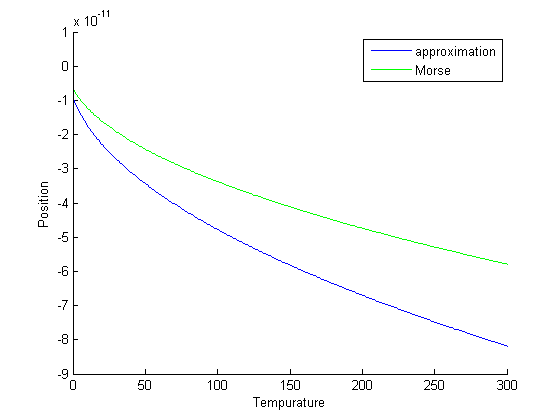
\includegraphics[width=0.8\textwidth]{temp.png}
  \caption{thermal dependence}
\end{figure}
As temperature increases, the lattice vibrates more and the position of the particle moves further away from zero on average. The curves look the same but diverge as temperature increases
%%----------------------------------------------------------------------------------------
%%	PROBLEM 4
%----------------------------------------------------------------------------------------
\section{\small{Molecular Simulation of Dynamical Systems}}
%%%%%%%%%%%%%%
\subsection*{\small{A) Plot of the potential function V(x) vs. x. How many equilibrium points can you identify if the particle moves according to this potential? Which ones are stable
equilibrium positions (e.g. particle will return to this position if perturbed
slightly).}}
\begin{figure}[H]
  \centering
      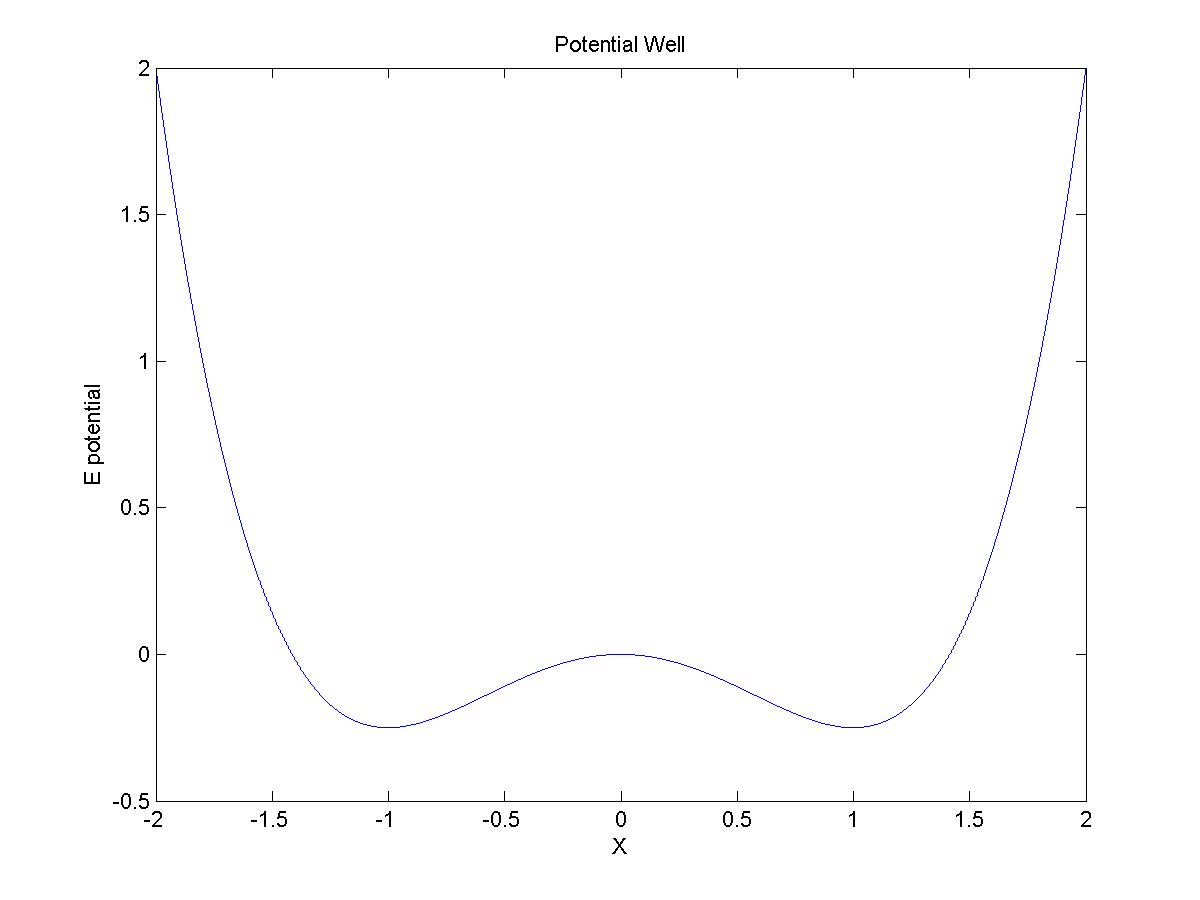
\includegraphics[width=0.8\textwidth]{Well.png}
  \caption{Well potential}
\end{figure}
3 equilibrium points. 2 stable equilibrium points.
%%%%%%%%%%%
\subsection*{\small{B) Write down the equation of motion for this particle under the given potential and dissipative force using Newton’s Second Law.}}
\[ V(x) = - \frac{x^2}{2} + \frac{x^4}{4}\] 
\[F(x) = -\frac{\partial V(x)}{\partial x}\]
\[F(x) = x + x^3\]
\begin{center}
\boxed{F(x) = x - x^3}
\end{center} 
%%%%%%%%%%%%
\subsection*{\small{C) Numeric Integration}}
i)
ii)
\begin{figure}[H]
  \centering
      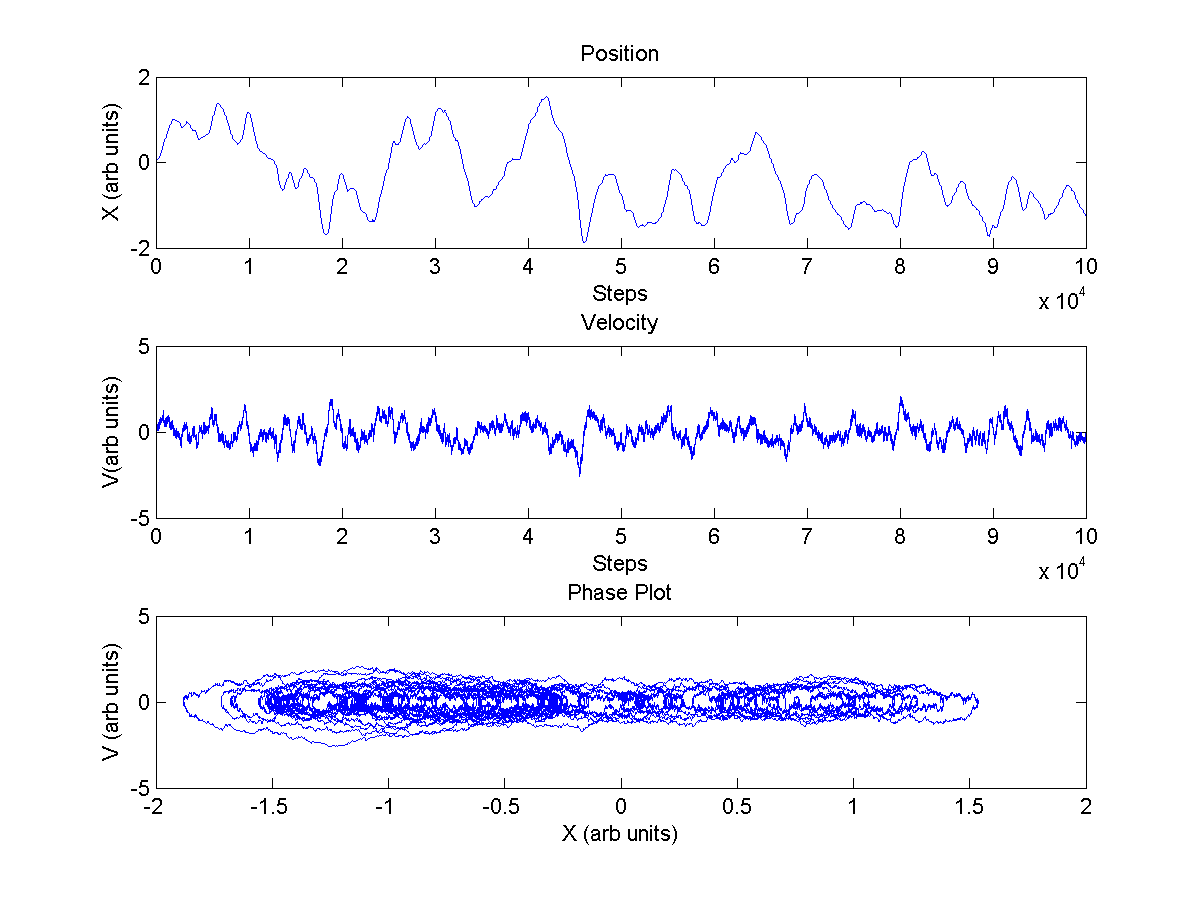
\includegraphics[width=0.8\textwidth]{ParticleMotion.png}
  \caption{A) Position B) Velocity C) Phase}
\end{figure}
iii)
\begin{figure}[H]
  \centering
      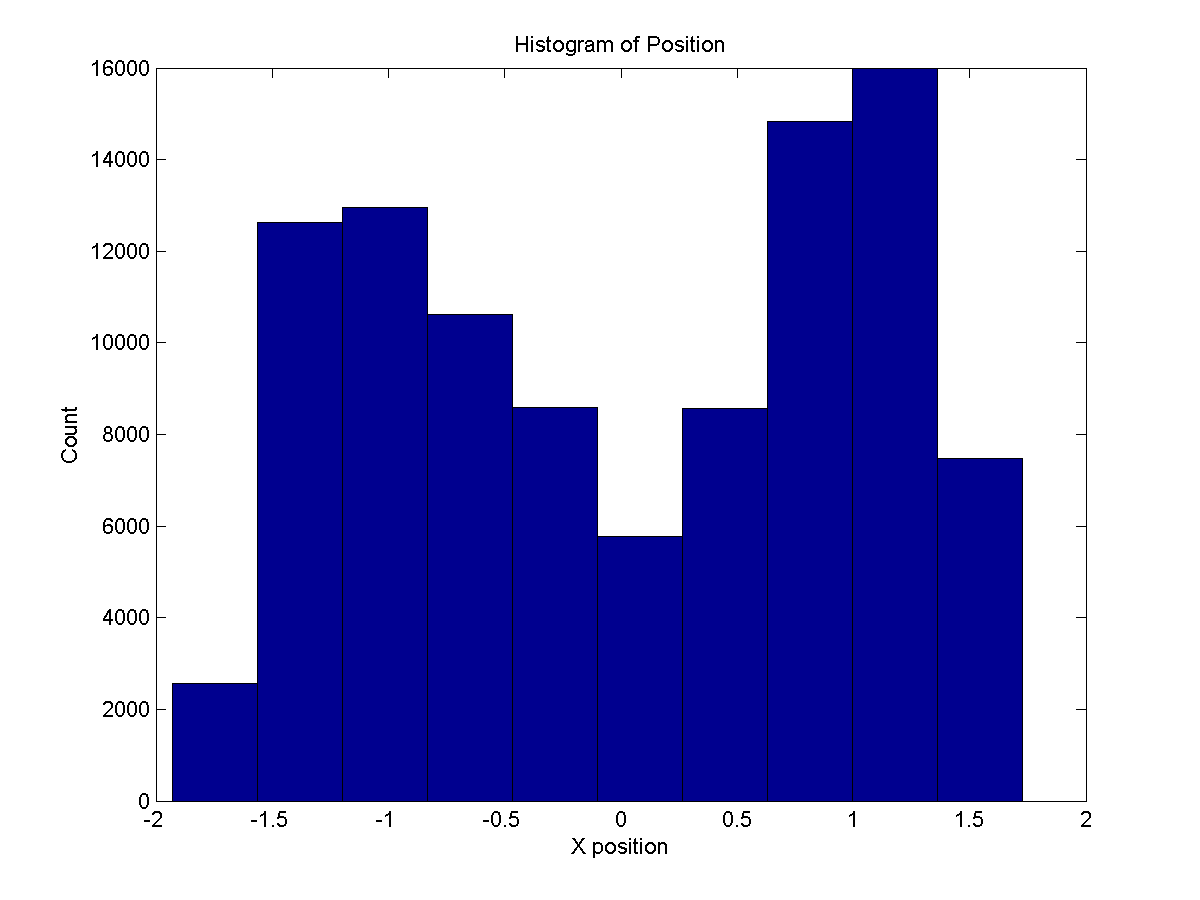
\includegraphics[width=0.8\textwidth]{HIST.png}
  \caption{Histogram of position}
\end{figure}
Peaks are observed at the valleys of the potential. The dissipative force \(F_D\) controls the probability distribution of the peaks.
iv) 
\[\tau_{Dwell} = 10.63 seconds\]
v)
\[ V''(\pm1) = K\]
\[V''(x) = -1 + 3x^2\]
\[K = 2\]
vi)
\subsection*{\small{D )Brownian Dynamics technique}}
i) I think that the particle will become trapped on one of the wells and stay there. \(\tau_{Avg}\) is dependent on the relation between \(K_b T\) and the barrier potential\\
ii) \(\gamma = 0\)\\
iii) 
\begin{figure}[H]
  \centering
      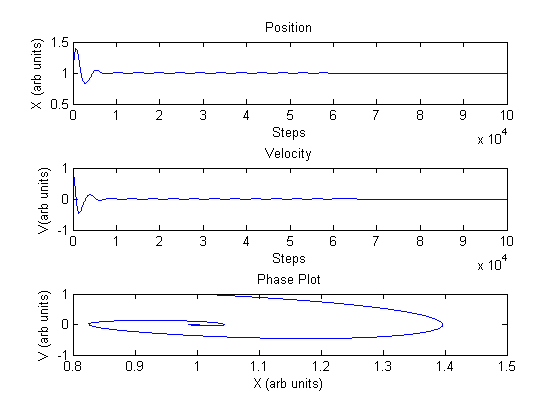
\includegraphics[width=0.8\textwidth]{iii1.png}
  \caption{\(\gamma = 1\)}
\end{figure}
\begin{figure}[H]
  \centering
      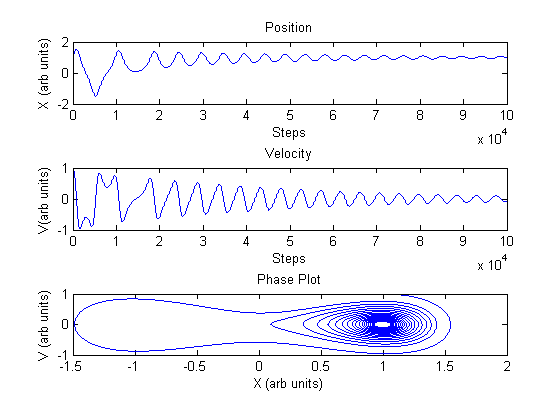
\includegraphics[width=0.8\textwidth]{iii005.png}
  \caption{\(\gamma = 0.05\)}
\end{figure}

%----------------------------------------------------------------------------------------
\subsection*{Matlab Code}
\lstinputlisting{HW1_416.m}
\lstinputlisting{molsim.m}
\lstinputlisting{part3.m}
\end{document}